\documentclass[a4paper, twoside]{article}

\usepackage{hyperref}
\usepackage[pdftex]{graphicx}
\usepackage{exercise}
\usepackage{mathtools}
\newcommand{\HRule}{\rule{\linewidth}{0.5mm}}


\begin{document}
\pagestyle{empty}

\begin{titlepage}

\begin{center}

\textsc{\LARGE Summerschool 2012}\\[1.5cm]

% Title
\HRule \\[0.4cm]
{\huge \bfseries Introduction into Robotics}\\
\HRule \\[1.5cm]

{\large
Mogelijk gemaakt door:\\
Het Dutch Nao Team\\
\url{http://dutchnaoteam.nl}\\[1.5cm]}

% Author and supervisor
\begin{minipage}{0.4\textwidth}
\begin{flushleft} \large
\emph{Auteurs:}\\
T. Blankevoort \\
D. Ten Velthuis \\
H. van der Molen \\
\end{flushleft}
\end{minipage}
\begin{minipage}{0.5\textwidth}
\begin{flushright} \large
\emph{In samenwerking met:} \\
Universiteit van Amsterdam\\
Technische Universiteit Delft\\
\indent \\
\end{flushright}
\end{minipage}

\vfill

{\Large \textit{Juli 2012}}
\end{center}
\end{titlepage}

\cleardoublepage
\begin{center}
Tijmen Blankevoort \\
Duncan Ten Velthuis \\
Hessel van der Molen \\
\indent \\
\indent \\
Dutch Nao Team\\
\url{http://dutchnaoteam.nl}\\
\indent \\
\indent \\
Versie 1.0 - Juli 2012\\
\indent \\
\end{center}

\cleardoublepage

\section*{Voorwoord}

\cleardoublepage


\tableofcontents{}

\cleardoublepage

\pagestyle{plain}
\setcounter{page}{1}
\section{Hello World}
\subsection{Introductie}
In deze opdracht gaan we de Nao ``Hello world'' laten zeggen, en maak je kennis met de opzet van de code.

Komende dagen zul je gaan werken binnen een framework van verschillende bestanden. Dit doen we zodat het project goed overzichtelijk blijft. Het framework bestaat zodoende uit verschillende modules. Ter referentie mag je de bijgevoegde readme lezen (zie appendix). Het is belangrijk dat je de volgende drie dingen en hun functies kent:
\begin{itemize}
\item config.py - start de code
\item module - Een class die code bevat. Moet minimaal de functie \textit{setDependencies(self, modules)} hebben.
\item main-module - Zelfde als een module, maar bevat minimaal de functies \textit{setDependencies(self, modules)} en \textit{start(self)}. Deze word als eerst aangeroepen.
\end{itemize}

Het aanroepen van config.py start de code. Een module is niks anders dan een verzameling code en functies die onafhankelijk van de andere code kan opereren. De code die jullie gaan schrijven bestaat uit modules voor de verschillende dagen, en uit modules die wij voor je hebben geschreven. Het opsplitsen van code op deze manier zorgt voor een duidelijke structuur en goed overzicht. We gaan nu eerst kijken hoe jullie zelf een module kunnen maken.

\subsection{Het framework}
\subsubsection{De main-module}
Open een nieuw document in Notepad++, noem het \textit{main.py} en sla het op in de map \textit{modules} van het geleverde framework. 
Een module begint met een klasse-naam gelijk aan zijn bestandsnaam. Een main-file bevat daarnaast ook minimaal 2 functies: \textit{setDependencies} en \textit{start}. \textit{setDependencies} word gebruikt om aan te geven welke modules gebruikt worden door deze module. \textit{start} word aangeroepen als main.
Omdat de functies op dit moment nog geen inhoud hebben, moet je het commando \textit{pass} onder de functie-declaratie geven. Het bestand zou er nu als volgt eruit moeten laten zien:

\noindent \line(1,0){100}
\begin{verbatim}
class main:
    def setDependencies(self, modules):
        pass

    def start(self):
        pass
\end{verbatim}
\noindent \line(1,0){100}
\\\\
Vergeet niet het bestand op te slaan!

\subsubsection{Een molule voor globale variabelen}
Binnen het framework zullen meerdere variabelen straks gedeeld worden door meerdere modules. Denk bijvoorbeeld aan het ip-adres van de Nao. Daarom is er een module nodig die deze variabelen en functies bevat.

Open een nieuw document in Notepad++ en noem het \textit{globals.py}, sla het op in de map \textit{modules} en geef het de juiste klasse-naam en functie(s). 

Een robot wordt aangeroepen aan de hand van zijn ip-adres. Dit is het adres dat de Nao heeft op het lokale netwerk. Start je Nao op en achterhaal zijn ip-adres op door op zijn chest-button te drukken. Dit ipadress moet als string worden genoteerd in de globals-module: \textit{ ipadres = "$<$ipadres-van-je-nao$>$"}. De variabele moet worden gezet in de globale scoop van de module, direct onder de definitie van de klasse.

Op de Nao zelf draait software die je aan kan roepen. Deze software heeft de naam Naoqi en is in wezen de `ziel' van de NAO.
Binnen de Naoqi worden Naoqi-modules aangeroepen via een proxy. Dit is een module die ervoor zorgt dat je over het netwerk de verschillende functies op de NAo aan kan roepen. Deze proxy genaamd ALProxy maken we als volgt aan in python: (\textit{from naoqi import ALProxy}). Om slechts 1 keer verbinding te maken met alle proxies defineren we een functie, \textit{setProxies(self)}, die dit doet. Deze functie zal straks door de main-module worden aangeroepen.

De Nao beschikt over een module die ervoor zorgt dat de Nao tekst kan oplezen. Dit is de `TextToSpeech-module'. Deze is aan te roepen doormiddel van: \textit{ALProxy(``ALTextToSpeech", self.ipadress, 9559)} \footnote{Je zult je wellicht afvragen waarom \textit{self} aan de globale variabele en aan functies is gekoppeld. Heel kort gezegt refereert het commando \textit{self} naar zijn eigen klasse. Python weet hiermee dat de informatie die het zoekt in de scoop van de eigen klasse zit.}. We willen dat de andere code die je schrijft deze naoqi-module kan aanroepen, dus slaan we de zojuist gemaakte referentie op in de variabele \textit{self.speechProxy}. De globals module heeft op deze manier een enkele verbinding met de Nao, en elke module die deze globals module als `dependency' heeft kan deze ook gebruiken.

Je code zou er nu als volgt uit moeten zien:

\noindent \line(1,0){100}
\begin{verbatim}
from naoqi import ALProxy
class globals:
    ipadres = "<ipadres-van-je-nao>"

    def setDependencies(self, modules):
        pass

    def setProxies(self):
        self.speechProxy = ALProxy("ALTextToSpeech", self.ipadres, 9559)
\end{verbatim}
\noindent \line(1,0){100}

\subsubsection{Het configuratie-bestand}
De zojuist gemaakte modules moeten nu nog worden geregistreerd in het framework. Hiervoor is er een bestand config.py. Dit is de file die je aan zal roepen om je code te draaien en bevat alle informatie over alle modules. Open dit bestand nu in Notepad++.

Als eerste moet de main-module worden geregistreerd. Zoals in de readme beschreven, wordt dit gedaan door:
 \textit{moduledict[``main"] = ``$<$class-name-of-module$>$" }. 
Omdat wij onze main-module \textit{main} hebben genoemd, ziet de registratie er uit als: \textit{moduledict[``main"] = ``main"}.
Registratie wordt gedaan vanaf regel 17 en voor het stuk dat het framework importeert en uitvoert.

Ook de globals-module moet worden geregistreerd. Om overzicht te houden is het slim om de referentie naam \textit{``globals"} te geven. Aan de hand van deze naam kunnen straks andere modules `globals' aanroepen en zijn informatie opvragen. De module naam is ook ``globals", daarom ziet deze registratie er als volgt uit: \textit{moduledict[``globals"] = [1, ``globals"]}


\textit{config.py} zou er nu ongeveer zo uit moeten zien:

\noindent \line(1,0){100}
\begin{verbatim}
# @file config.py
# @func module definitions for framework. 
#       Is used to register, define & load modules 
#       Starts the main-framework
# @auth Hessel van der Molen
#       hmolen.science@gmail.com
# @date 4 may 2012

#dictionary for module
moduledict = {}
#show frameworks print's (1=show, 0=do not show)
VERBOSE = 1

####
## Register modules:
#######

moduledict["main"] = "main"
moduledict["globals"] = [1, "globals"]

###########################
# start & run framework
###########################
from framework import mframework
mframework.startUpFramework(moduledict, VERBOSE)
\end{verbatim}
\noindent \line(1,0){100}

\subsection{Hello World}
Het framework (en je code) is nu klaar om te runnen. Dit wordt gedaan door het programma \textit{Command Prompt} (All Programs $>$ Accessories) te openen. 
Ga nu behulp van de commando's ``cd"  en ``dir" naar de map waar \textit{config.py} staat.
Door \textit{python config.py} te typen wordt de code gestart.

Start de code en bekijk wat er gebeurd.

Als het goed is, sluit het systeem (na enkele prints te hebben gedaan) netjes af. Dit klopt, aangezien onze main nog geen code uitvoert.

Om het Hello World-voorbeeld af te maken moeten we weer terug gaan naar onze main-module.

De main-module is afhankelijk (dependent) van de globals. Daarom moet de \textit{globals}-module via \textit{setDependencies(self, modules)} worden aangeroepen:

\noindent \line(1,0){100}
\begin{verbatim}
def setDependencies(self, modules):
    self.globals = modules.getModule("globals")
\end{verbatim}
\noindent \line(1,0){100}
\\\\
Via de variabele \textit{self.globals} hebben we in de main-module toegang tot alle globale data.

Om iets met de Nao te kunnen doen moeten de proxies worden gemaakt om informatie over te sturen. Dit doen we nu met de code \textit{self.globals.setProxies()}. Dit dient natuurlijk te gebeuren nadat de code is opgestart (na \textit{start(self)} is aangeroepen door het framework).
Wanneer de proxies zijn aangeroepen kunnen we gebruik maken van de variabele \textit{speechProxy} uit \textit{globals}.
Met behulp van het commando \textit{say(``Text...")} kan de Nao Engelse text uitspreken. In ons systeem ziet dit er als volgt uit:

\noindent \line(1,0){100}
\begin{verbatim}
def start():
    self.globals.setProxies()
    self.globals.speechProxy.say("Hello World")
\end{verbatim}
\noindent \line(1,0){100}
\\\\
Sla alle code op en run opnieuw \textit{config.py}. Gefeliciteerd! Je Nao heeft iets gezegd! Hiermee heb je nu voor de eerste keer verbinding gelegd met de Nao om hem een instructie te geven.


\cleardoublepage
\section{Behaviour}
Maak behaviour module aan...

Nu gaan we de Nao laten bewegen.
In de map \textit{lib} in \textit{modules} staan enkele modules gedefineerd die je kan gebruiken gedurende deze summerschool.
Voor de volgende opdracht heb je de module \textit{motion\_v1.py} nodig.

\subsection{Lopen}
\subsubsection{De motion-module}
Deze module verwacht de proxies motProxy en posProxy in de globals-module. De \textit{motProxy} zorgt voor een verbinding met de motoren, zodat de robot kan worden aangestuurd. \textit{posProxy} wordt gebruikt om de robot positie (de stand van de motoren) uit te lezen. Als eerste moet de \textit{globals} module worden uitgebreid met een aanroep naar deze proxies, zoals we eerder met TextToSpeech hadden gedaan.
Voeg aan de \textit{setProxies(self)} functie de volgende code toe:

\noindent \line(1,0){100}
\begin{verbatim}
self.motProxy = ALProxy("ALMotion", self.ipadres, 9559)
self.posProxy = ALProxy("ALRobotPose", self.ipadres, 9559)
\end{verbatim}
\noindent \line(1,0){100}
\\\\

Naast het aanpassen van de \textit{globals}-module, moet ook \textit{config.py} worden geupdate en de main-module moet de motion-module kunnen inladen.
In de main-module, nadat de proxies zijn geladen, moet de \textit{init(self)} functie van de motion-module worden aangeroepen. Deze functie zorgt ervoor dat de juiste parameters voor bewegingen worden geladen.

Voeg bovenstaande functionaliteit zelf toe aan je code en test het daarna. Zorg ervoor dat je alle errors oplost voordat je verder gaat! (waarschuwingen zijn geen probleem). De code moet aangeven dat het framework goed is geladen/afgesloten!

\subsubsection{WalktTo() en setWalkTargetVelocity()}
Bekijk nu eens alle functies die in de motion-module staan, zodat je een globaal idee hebt wat je er allemaal mee kan doen.

Voordat je begint met het beweten is het belangrijk te weten dat hiervoor de motoren aan moeten staan. Dit heet 'stiffness'. Als de motoren 'stiff' zijn kan je de Nao zelf niet meer bewegen. De motoren van een Nao raken snel oververhit, zorg er dus voor dat als je hem niet gebruikt dat de sitffness uit staat. Dit kan je doen door twee keer snel op de buik-knop te drukken.

Voordat de robot kan lopen moet hij eerst opstaan, en moeten de motoren aan staan. Dit kan gedaan worden met de functie \textit{standUp(self)}.

Deze functie test zelf als de robot is gevallen, als dat het geval is laat het de robot opstaan en anders doet het niks.
Om te lopen zijn de functies \textit{walkTo(x, y, angle)} en \textit{setTargetVelocity(x, y, angle, frequency)} beschikbaar.
Met de eerste functie loopt de robot de opgegeven afstand, terwijl bij de tweede optie de robot een richting op loopt, en blijft lopen.

Je hebt nu alle benodigdheden om de Nao te laten lopen! Maak, door middel van onderzoek hoe de loop-functies werken, nu functies die het volgende doen:
\begin{itemize}
\item Loop een vierkant: 1 meter naar voren, 1 meter naar links, 1 meter naar achteren en 1 meter naar rechts
\item Loop een vierkant: 1 meter naar voren, draai 90 graden, loop naar voren, et cetera.
\item Loop een rondje van ca 1 meter doorsnee.
\item Loop door het doolhof heen.
\end{itemize}

Extra noties en tips:
\begin{itemize}
\item Als de robot valt tijdens het lopen, moet deze opstaan en het figuur afmaken.
\item Tip: Zoek eerst uit hoe de loop-functies werken en hoe ze aan te roepen zijn. Test vooral veel!
\item Tip: Het kan handig zijn om vier verschillende main-modules te maken, elk voor een apart loopje. Met behulp van \textit{config.py} kun je andere main-modules inladen en zo wisselen tussen loopjes.
\item Tip: Als je meerdere modules gaat maken, is het handig om dit netjes in mappen te plaatsen zodat je overzicht houd.

\item Tip: Hoewel all nodige motions in de motion module staat, kun je met behulp van de \textit{motProxy} direct motion-behaviours aanroepen uit nao-qi. De documentatie hiervoor kun je vinden door ``Nao reference" op je bureaublad aan te klikken. Daarna ga je naar: ``NAOqi API $>$ ALMotion". 
\end{itemize}

\subsection{Ball tracking}
\subsection{Tips}

\cleardoublepage
\section{Vision}
\subsection{Introductie}
Voor de vision opdrachten maken we gebruik van Open CV \footnote{Voor documentaties, zie: \\ \url{http://opencv.willowgarage.com/documentation/python/index.html}}. Dit is een Computer Vision library die door meerdere programmeertalen kan worden gebruikt voor beeld verwerking.

\subsection{Framework-update}
Om de robot de weg te laten vinden, moet deze gebruik maken van zijn camera. Een Nao heeft 2 camera's in zijn hoofd zitten: \'e\'en in zijn mond en \'e\'en in zijn voorhoofd. Wij zullen enkel de camera in de mond gebruiken.

Net als bij motions wordt de camera ook via een proxy aangeroepen. Door \textit{self.vidProxy = ALProxy( ``ALVideoDevice", self.ipadres, 9559 )} toe te voegen aan de \textit{setProxies()} functie krijgen we de mogelijkheid om te camera uit te lezen. Voordat we een foto kunnen maken moeten er nog enkele camera parameters worden ingesteld. Dit wordt gedaan door de \textit{cSubscribe()} functie in de \textit{tools}-module.

Vergeet niet, voordat je verder gaat, het juiste ip-adres van de robot door te geven aan de globals-module.

\subsubsection{tools}
over tools-module..

\subsection{Blob-detectie}
De eerste stap in het navigeren door ons doolhof is het vinden van een blob: een gebied in een plaatje dat \'e\'en bepaalde kleur heeft. In de komende secties zul je je eigen blob-vinder maken.

\subsubsection{Een foto maken en opslaan}
Met behulp van de \textit{getSnapShot()} functie in de tools-module kun je een foto maken met de onderste camera van de robot. Deze functie geeft naast de foto ook extra gegevens terug over de positie van het hoofd. Het eerste argument van de geretourneerde waarde van \textit{getSnapShot()} is het plaatje.

Een gemaakt plaatje kan ook worden opgeslagen. Dit wordt gedaan door de functie \textit{saveImage(name, img)} aan te roepen in de tools-module. Hierin is \textit{name} de bestandsnaam (een string dus) van het plaatje inclusief de bestands-extensie (png of jpg). \textit{img} is het plaatje zelf.

Maak een plaatje en sla dit op. Het opgeslagen bestand kun je vinden in de zelfde map als waar je \textit{config.py}-bestand staat.

Wanneer je het plaatje opent, zul je zien dat de kleuren niet kloppen. Dit klopt, wij gebruiken namelijk de HSV-kleuren\footnote{Meer informatie over HSV kun je vinden op: \\ \url{http://nl.wikipedia.org/wiki/HSV_(kleurruimte)} } representatie in plaats van de wat bekendere RGB-representatie. Zoek deze representatie op op wikipedia zodat je begrijpt wat de componenten Hue, Saturation en Value zijn.

\subsubsection{Image filtering}
Een volgende stap in het proces is het filteren van een kleur. Hiervoor moet een functie worden gemaakt die een snapshot en enkele kleur-parameters meekrijgt en een gefilterd zwart/wit plaatje terug geeft. In dit gefilterde (binaire) plaatje staan witte pixels voor pixels welke in de meegegeven foto voldoen aan onze kleur-eisen en zwarte pixels staan voor pixels die hier niet aan voldoen.

Voordat code kan worden geschreven moet een module worden gemaakt waar straks de code in komt te staan (de \textit{vision}-module). Deze module kun je vinden in de map \textit{vision}. De module is aangemaakt, maar wordt nog niet ingeladen (zie \textit{config.py}). De \emph{main}-module heeft de \textit{vision} module nodig, pas daarom ook \textit{setDependencies} aan in de \emph{main}-module.
Zoals je kan zien importeert de \textit{vision} module verschillende libraries, onder ander \textit{cv} en \textit{cv2}, dit zijn de gebruikte OpenCV bestanden.

De eerste functie die in \textit{vision}-module moet worden geimplementeerd is de \textit{filterImage(self, img, minHSV, maxHSV)}-functie.
Als input krijgt het een plaatje mee en twee lijsten met elk 3 waardes (minimum en maximum waardes van de Hue, Saturation en Value van een kleur). Pixels in het plaatje die binnen deze kleur-grenzen vallen zijn pixels waarin we interesse in hebben. Dit is te vergelijken met bijvoorbeeld een beschrijving van elke kleur die minimaal lichtblauw is en maximaal donkerblauw. Op deze manier kunnen we alle blauwe kleuren markeren en daarmee vinden we de pixels die voor ons interessant zijn.
Om OpenCV te kunnen laten werken met de kleur-definities moeten we de lijsten met HSV-waardes omzetten in een Scaler (constante waarde):

\noindent \line(1,0){100}
\begin{verbatim}
minScaler = cv.Scaler(minHSV[0], minHSV[1], minHSV[2], 0)
\end{verbatim}
\noindent \line(1,0){100}
\\\\
Het omzetten moet voor beide lijsten (\textit{minHSV} en \textit{maxHSV}) worden gedaan. Het eerste argument, \textit{minHSV[0]} is de Hue-waarde van de ondergrens van de gewenste kleur. Het tweede argument, \textit{minHSV[1]}, is de Saturation en het derde, \textit{minHSV[2]}, de Value. Het omzetten van de lijst van \textit{maxHSV}-waardes gebeurt op eenzelfde manier.

Uiteindelijk zal onze filter-functie een nieuw plaatje terug geven. Om dit te kunnen doen moet geheugen worden vrijgemaakt:

\noindent \line(1,0){100}
\begin{verbatim}
resultImg = cv.CreateImage(size, cv.IPL_DEPTH_8U, 1)
\end{verbatim}
\noindent \line(1,0){100}
\\\\
Hierin is \textit{size} gelijk aan \textit{(320,240)}, de grootte van de gemaakte foto. \textit{cv.IPL\_DEPTH\_8U} geeft aan dat elke pixel uit het plaatje een 8-bit unsigned waarde heeft (integers tussen 0 en 255. Het aantal dimensies (kleuren) van het plaatje is 1: een pixel is enkel zwart of wit.

We kunnen nu OpenCV gebruiken om een `raw' zwart-wit plaatje te maken van de kleuren in onze foto:

\noindent \line(1,0){100}
\begin{verbatim}
cv.InRangeS(img, minScaler, maxScaler, resultImg)
\end{verbatim}
\noindent \line(1,0){100}
\\\\
Onze filter creert nu al een resultaat. Return het resultaat en roep de functie vanuit de \textit{main}-module aan met een kleur naar keuze (zie voor HSV-waarders het whiteboard). 
Het resultaat kunnen we als een plaatje opslaan met behulp van de eerder genoemde \textit{SaveImage}-functie. Zorg evoor dat het resultaat van de filter-functie wordt opgeslagen. Sla dan al je code op, test het, los eventuele errors op en bekijk het resultaat.

Hoogst waarschijnlijk zul je vele witte vlekken zien in plaatje. Dit is meestal ruis en komt door de kwaliteit van de camera en mogelijk kleuren in ed achtergrond. Om dit weg te halen moeten we het plaatje ``smoothen": de overgang tussen zwart/wit maken we minder `hard'. Voor elke pixel kijk je naar zijn buren, als er meer witte dan zwarte buren zijn zet de functie de pixel op wit, en anders op zwart. Random witte pixels zullen daardoor een zwarte kleur krijgen en dus wegvallen. De volgende functie doet dit: \textit{cv.Smooth(resultImg, resultImg, cv.CV\_MEDIAN, 1)}. \textit{cv.CV\_MEDIAN} geeft het type ``smoothing" aan en het getal hoeveel naastelkaar gelegen pixels steeds worden gebruikt per berekening. Voeg deze functie toe in je filter-functie en pas je return aan zodat het gesmoothte plaatje terug wordt gegeven. 
Run je code en test een paar verschillende waardes om te bepalen welk getal het beste resultaat geeft\footnote{Op \url{http://opencv.willowgarage.com/documentation/python/image_filtering.html\#smooth} kun je meer vinden over de mogelijke opties van smoothing.}.

De filter functie heeft nog 1 toevoeging nodig: het plaatje moet worden omgezet in een ander formaat zodat andere functies straks verdere bewerkingen kunnen doen. Het omzetten wordt gedaan met het commando: \textit{resultImg = cv.GetMat(resultImg)}. Voeg deze optie toe en test je code op fouten.

\subsubsection{Hough Circels}

Nu we een gefilterd plaatje krijgen, kunnen we proberen cirkels te zoeken. Hiervoor is een nieuwe functie nodig in onze vision-module. Deze functie heeft (naast \textit{self}) slechts 1 argument: een binair plaatje (\textit{findCircle(self, img)}

Cirkel detectie doen we doormiddel van een speciaal algorithme: de Hough-transform\footnote{voor meer info check: \url{http://en.wikipedia.org/wiki/Hough_transform}}. Dit algorithme komt met OpenCV geleverd. Om de Hough-transform te kunnen toepassen moet het gegeven plaatje worden omgezet in een array via \textit{numpy} (een python module): \textit{img = numpy.asarray(img)}. De library is (zoals je kan zien) al geimporteerd bovenaan het begin van de vision-klasse.

Na het vekrijgen van een plaatje, moet de functie de Hough-transform toepassen. Hier komen echter veel verschillende parameters bij kijken. Om ervoor te zorgen dat je niet te veel tijd kwijt bent aan het tweaken hiervan geven wij je de ``juiste" parameters:

\noindent \line(1,0){100}
\begin{verbatim}
dp = 2
minD =120
p1 = 255
p2 = 27
minS = 8
maxS = 300
circles = cv2.HoughCircles(img, cv.CV_HOUGH_GRADIENT, dp, minD, None, p1, p2, minS, maxS)
\end{verbatim}
\noindent \line(1,0){100}
\\\\
\textit{dp} geeft aan hoe nauwkeurig moet worden gezocht (in ons geval om de 2 pixels), \textit{minD} geeft aan hoeveel pixels minimaal tussen 2 blobs moet zitten, \textit{p1} en \textit{p2} zijn parameters voor een dieper-liggend proces en \textit{minS} en \textit{maxS} geeft aan wat de minimale, danwel de maximale grote van een blob is in pixels.
De output is een lijst met daarin data over de gevonden cirkels (aantal, radius, pixel-center), of \textit{None} indien niks gevonden is.

Sla je code op en test de \textit{HoughCircles} functie. Print het resultaat van de aanroep in de Command Prompt. 

Aan de hand van de geprinte data, kun je nu een systeem maken welke \textit{None} terug geeft als geen cirkel is gevonden of een lijst met coordinaten als er wel cirkels zijn gevonden.

\begin{itemize}
\item Tip: De \textit{HoughCircles}-functie kan meerdere cirkels terug geven. \textit{len(circles[0])} geeft je het aantal gevonden cirkels. De straal en centrum (x en y) van de $i${de} cirkel van de lijst is te vinden met respectievelijk \textit{circles[0][i][2]}, \textit{circles[0][i][0]}, \textit{circles[0][i][1]}
\item Tip: Met behulp van het commando: \textit{cv.Circle(img, center, radius, (0, 0, 255), 3, 8, 0)} kun je een cirkel met centrum \textit{center} en straal \textit{radius} teken op het plaatje img. Wanneer je het plaatje opslaat kun je visueel zien waar het algorithme denkt dat de blobs zitten.
\end{itemize}

\subsubsection{Meerdere blobs}
Nu we blobs kunnen herkennen en berekenen waar ze in een plaatje zitten, kunnen we meerdere blobs combineren.

Hiervoor is een functie nodig (in de vision-module, \textit{getBlobsData(self, img)}) die een plaatje inlaad (geven door de main-module, via \textit{getSnapshot()}), die voor elke kleur blob detectie doet en vervolgens zoekt  naar Hough-Circles. De functie moet 2 outputs geven, de eerste is het aantal gevonden blobs, de tweede is een lijst met daarin de co\"ordinaten (op volgorde) van de paarse, blauwe en oranje blob. Als er geen co\"ordinaten van een blob zijn gevonden dan staat er \textit{None} op deze plek. 

Het is belangrijk dat je gedurende het programma steeds dezelfde volgorde van blobs aanhoud in je lijst: \textit{[paars, blauw, oranje]}. Test je code zorgvuldig zodat je weet dat dit het geval is.

\subsection{Tips}
tips..


\cleardoublepage
\section{Vision \& Behaviour}
\subsection{Landmark Detectie}
Gefeliciteerd, als je hier ben aangekomen zul je een werkende vision module hebben die blobs kan vinden.

\subsubsection{Afstand en Hoek schatten}
De volgens stap is de mapping van de gevonden blobs naar een landmark en de berekening van de afstand en de hoek tot de landmark. Deze waardes gebruiken we om op de ``perfecte" plek te komen voor de landmark, zodat we netjes naar links of rechts kunnen draaien.

We beginnen met het berekenen van de afstand tot de landmark: je wilt de robot naar een landmark toe laten lopen en stoppen zodra hij op een bepaalde afstand van de landmark staat. Dit is simpel te doen door de afstand tussen de verschillende blobs te berekenen. Zoals je bij de vorige opdracht gezien hebt is het vision-systeem gevoelig voor ruis. Daarom bereken je een gemiddelde afstand tussen de blobs. Hiervoor moet de functie \textit{calcAvgBlobDistance(self, blobList)} worden gemaakt in de \textit{vision} module. Deze krijgt als input de lijst met gegevens van blobs. Als output wordt de gemiddelde afstand (in pixels) tussen de gevonden blobs terug gegeven. Bij 1 (of 0) blobs kan er geen afstand worden berekend, en wordt er \textit{None} geretouneerd.

Met deze code is het al mogelijk om op de juiste afstand te stoppen voor je landmark. Test je code en bepaal bij welke gemiddelde afstand de robot op de juiste afstand (ongeveer 44 cm) staat en laat de robot dan stoppen.

Voor het berekenen van de hoek naar een landmark, moet bekend zijn wat het midden van de landmark is. De functie die dit doet is \textit{calcMidLandmark(self, blobList)}. Als input krijgt het de lijst met gevonden blob-data en als output geeft het een x/y pixel positie die het midden aangeeft van de set van de gevonden blobs. Indien geen blobs zijn gevonden moet de functie \textit{None} terug geven.

Wanneer het midden van de set van blobs bekend is, kan de hoek ten opzichte van de robot worden berekend (\textit{calcAngleLandmark(self, center)}). Hiervoor gebruik je de volgende informatie:
De kijkhoek van de camera is ongeveer 70 graden (1.22 radialen). Een plaatje is 320 pixels breed, wat betekent dat een enkele pixel een hoek heeft van ongeveer 0.0038 radialen (1.22/320). Het midden van een plaatje heeft een hoek van 0 en een x/y pixel-positie van 160/120. \textit{None} moet worden geretouneerd wanneer geen blobs zijn gevonden en daarmee ook dus geen hoek kan worden berekend.

\subsubsection{Signature bepaling}
Als laatste stap moet een functie (\textit{findSignature(self, blobList)}) worden gemaakt die bepaald wat de signature is van de geobserveerde landmark. De signatures zijn als volgt verdeeld:

\begin{enumerate}
\item - Blauw boven, finish
\item - Blauw rechts, rechtsaf
\item - Blauw links, linksaf
\end{enumerate}

Indien een landmark niet kan worden bepaald, is de signature gelijk aan -1.

\subsection{Navigatie}
BEHAVIOUR MODULE\\
\\
\\
Het is nu mogelijk, gegeven een snapshot, om blobs te vinden, de afstand tussen de blobs te berekenen (en daarmee de afstand van de robot naar de landmark te schatten) en de hoek naar de gevonden blobs te berekenen. Verder kan (indien er alle blobs zijn gevonden) de signature van de landmark worden achterhaald.

Met al deze informatie kan de functie \textit{calcDirection(self, blobFound, blobDist, angle, signature)} worden gemaakt. Omdat dit geen vision-functie meer is, maar een behaviour moet een behaviour module worden aangemaakt.

De main module zal nu een snapshot maken, all vision functies aanroepen en de resultaten doorgeven aan de behaviour module. Deze module zorgt er dan voor, afhankelijk van de input, welke richting de robot op moet lopen of draaien. 
\\

Hoe zorg je ervoor dat je robot het snelst door het doolhof gaat?

\begin{itemize}
\item Tip: omdat je in een modulair systeem werkt kun je snel meerdere kopieen van je modules maken en laden. Hiermee kun je makkelijk kleine aanpassingen testen, zonder werkende code te verliezen
\item Tip: ALs je het makkelijker/mooier programmeren vindt kun je met behulp van simpele if-statements in je main bepalen wanneer het aanroepen van een functie wel of niet zin heeft.
\end{itemize}


\subsubsection{Stoppen..}
\subsubsection{en Draaien...}
\subsection{Tips}

\cleardoublepage
\section{Path-planning}
\subsection{Introductie}
Voor deze opdracht is het de bedoeling om een padplanner gebasseerd op het A* algoritme te maken\footnote{Zie wikipedia voor een beschrijvin van het algorithme en pseudo-code: \url{http://en.wikipedia.org/wiki/A*_search_algorithm}}.Met dit algoritme kan je de Nao straks met behulp van een kaart in \'e\'en keer met het kortste pad door het doolhof heen laten lopen. 

\subsection{Framework-update}
Om een map in te laden, en voor debugging staan in het framework 2 extra modules:
\begin{itemize}
\item mazeparser\_v1.py
\item visualizer\_v1.py
\end{itemize}

Je kunt deze modules gebruiken, maar je kunt ze ook zelf schrijven aan de hand van de interface-beschrijvingen (laatste is zeker aan te raden als je het leuk vind om te programmeren!).


\subsubsection{visualizer}
De visualizer bevat 3 functies: \\
\begin{itemize}
\item \textit{init()} - Deze functie initializeert de visualizer en moet daarom direct na de \textit{start()}-functie van je main-module worden aangeroepen.
\item \textit{stop()} - Voordat de \textit{start()}-functie is afgelopen, moet deze functie worden aangeroepen. Het zorgt ervoor dat de visualizer netjes afsluit.
\item \textit{visualize(edges, path, seen, start, end, scale=(100,100), offset=(100,100)))}\\ Hierin is \textit{edges} de dictionary van edges die bij de \textit{maxeparser} wordt terug gegeven. \textit{path} is een lijst van coordinaten waar het pad doorheen loopt.\textit{seen} is een lijst met nodes die al zijn bezocht. De \textit{start} en \textit{end} parameters zijn de begin en eind (goal) posities die de robot heeft. De \textit{scale} en \textit{offset} functies zijn ervoor om de grafische output op te schalen.
\end{itemize}

Om je A*-algoritme te debuggen, is het handig om steeds je huidige beste pad te printen. Dit is met de 3e functie van de \textit{visualizer}-module te doen. Om dit te kunnen doen moet je zorgen dat je A*-module de \textit{visualizer}-module mee neemt in zijn \textit{setDependencies}. Je kunt nu, door de \textit{visualize}-functie aan te roepen, in elke iteratie van het algoritme het huidige pad laten zien. Door in het venster  op `c' te drukken, gaat je algoritme een stap verder (het aanroepen van de visualizer is een ``blocking"-call).

\subsubsection{mapparser}
De mazeparser beschikt over 2 functies:
\begin{itemize}
\item \textit{parseMaze(filename="./maze.txt")} - Het argument filename is optioneel, als de functie als \textit{parseMaze()} wordt aangeroepen, dan wordt het .txt-bestand `maze.txt' geopend en ingelezen. De functie retourneerd 2 waardes. Het eerste is een dictionary van edges, het 2e een dictionary van geldige moves per cel. Een cel is gerepresenteerd als een tuple $(x,y)$, waarbij (0,0) links boven is en $x$ de horizontale richting aangeeft. Alle mogelijke moves vanuit een cel worden gezet in een lijst.
\item \textit{prettyPrint(edges)} - Als input wordt de dictionary \textit{edges} verwacht (gegeven door de bovenstaande functie). De ouput is een geprintte versie van het doolhof in je terminal.
\end{itemize}

\subsection{Het A*-star algoritme}
\subsection{Tips}
A* houdt een priority queue bij van de mogelijke incomplete paden in het doolhof. Deze zijn gesorteerd op de geschatte totale kosten om via elk pad het eindpunt te bereiken. Het pad met de laagste geschatte kosten heeft de hoogste prioriteit en staat vooraan in de priority queue. Als een pad wordt uitgebreid ontstaan er nieuwe paden die in de queue geplaatst moeten worden aan de hand van hun geschatte kosten. De library \textit{bisect} \footnote{Documentatie over \textit{bisect} op: \url{http://docs.python.org/library/bisect.html}.} kan gebruikt worden om een nieuw pad op de juiste plaats toe te voegen in de priority queue:\\
\noindent \line(1,0){100}
\begin{verbatim}
import bisect
...
bisect.insort(queue, newPath)
\end{verbatim}
\noindent \line(1,0){100}
\\\\
Het is hierbij van belang hoe \textit{newPath} gerepresenteerd wordt. Als \textit{newPath} een Tuple is dan zal het toegevoegd worden aan de hand van het eerste argument in de Tuple; bij een List aan de hand van het eerste argument in de List. Het is daarom van belang dat de geschatte totale kosten van een pad het eerste argument is in het gekozen datatype. 
\\
\\
KAN OOK MET HET COMMANDO \textit{min}, indien je een lijst hebt met tuples, waarvan een tuble is gerepresenteerd als: (total estimeted cost, cost so far, [path...]).
\cleardoublepage

\section{Path-planning in de ``Echte Wereld"}
\subsection{Introductie}
Nu jullie A* planningsalgoritme af is zouden jullie de robot bij een willekeurige ingang kunnen zetten, en de robot intrueren om naar een willekeurige uitgang te lopen! Alleen weet de robot nog niet waar hij is in het doolhof. Jullie zouden net als bij dag 2 de kleurenmarkers kunnen gebruiken op de muur om zo te bepalen waar je bent.Zoals je misschien al hebt gemerkt zijn deze kleurenmarkers vrij instabiel. Vandaag gaan we met stabielere landmarks werken die in de robotica veel worden gebruikt. Dit zijn Augmented Reality (AR) codes. Op het middelpunt van elke vierkant in de grid leggen we zo een AR code neer. Zo kan de Nao altijd stabiel zien waar hij naartoe loopt.

\subsection{Framework-update}
Schrik niet dat er een regeltje output in je python scherm komt, deze kan je gewoon negeren. Dit komt door het omzetten van de C$\stackrel{}{++}$ naar Python code. 
We gaan de code nu een klein beetje ontleden. Als eerste moeten de modules cv en cv2 geinclude worden (standaard voor computer vision AI software). Daarnaast gaan we numpy nodig hebben, dit is een python library die ervoor zorgt dat numerieke code erg snel uitgevoerd kan worden. Ook moeten we natuurlijk een ARimport class aanmaken. Dit gebeurd in de eerste 4 regels van ARtest.py.
\begin{itemize}
\item \emph{ARcode = ar.ARimport()} maken we een nieuw ARcode object aan. Tegelijk initialiseert deze regel ook dit object met al zijn nodige waardes.
\item \emph{image = cv.LoadImage("test.png",cv.CV\_LOAD\_IMAGE\_COLOR)} Laad het opencv testplaatje als kleurenplaatje
\item \emph{im\_array = np.asarray( image[:,:] ) } Om het plaatje naar de C$\stackrel{}{++}$ te kunnen sturen moeten we er een numpy array van maken.
\item{ARcode.setOutputFileName("output.png") / ARcode.setShowOutput(True)} Met deze regels zetten we de output van de library aan. Deze kan je in je uiteindelijke implementatie gewoon uit laten.
\item{returnint = ARcode.findMarkers(im\_array)} Als je deze functie aanroept gaat ARcode de markers berekenen, deze worden lokaal opgeslagen in de ARcode class. Hij returned een integer die aangeeft hoeveel markers er zijn gevonden.
\item{output = ARcode.getFoundMarker(0)} Deze functie geeft de informatie van de gevonden marker. Het getal dat je meegeeft is het nummer van de marker waar je de informatie van opvraagd. Dit getal mag niet groter zijn dan `returnint' dan crasht de applicatie gegarandeerd. met output.ID, output.x en output.y kan je de ID van de gevonden marker en de x en y positie in het gegeven plaatje van het midden van de marker vinden.
\end{itemize}

\subsubsection{AR-codes}

\begin{figure}[h]
\begin{center}$
\begin{array}{ccccc}
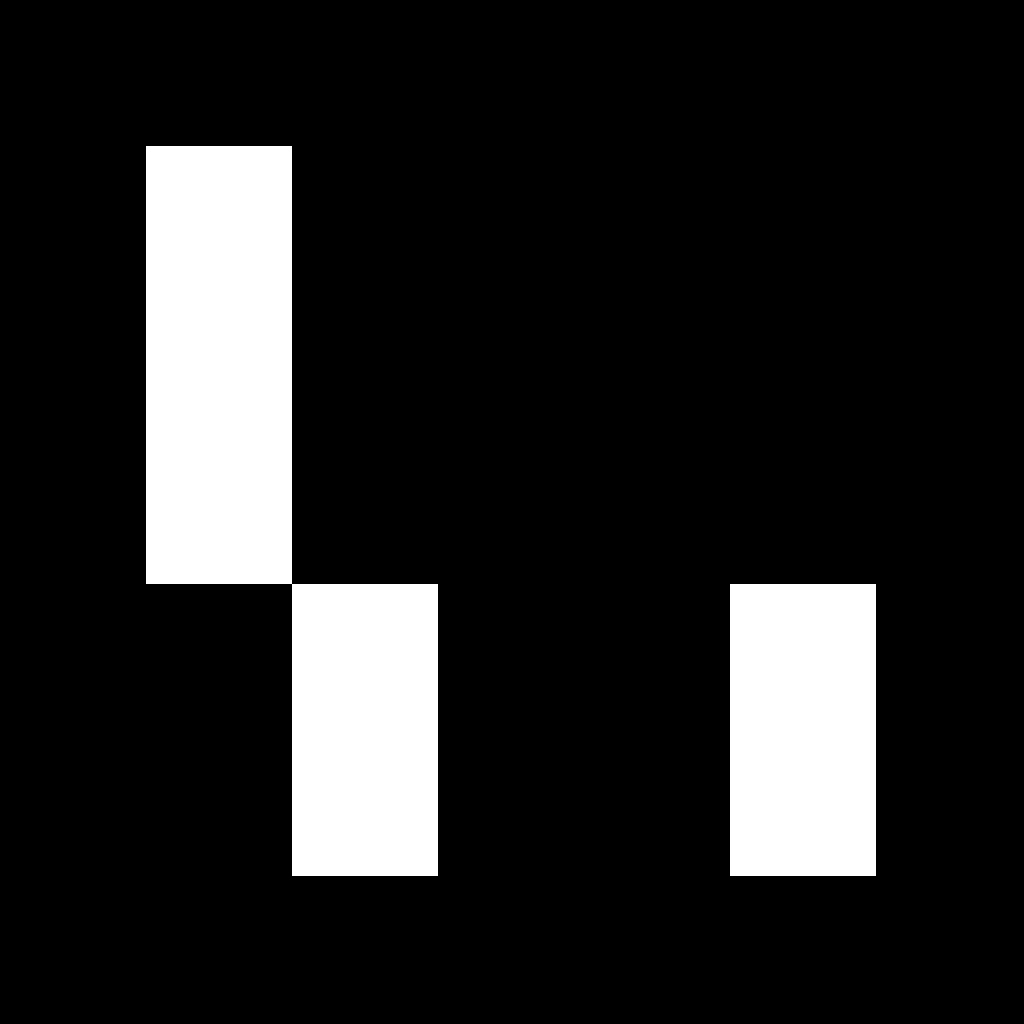
\includegraphics[width=0.8in]{img/10.jpg} &

\includegraphics[width=0.8in]{img/23.jpg} &

\includegraphics[width=0.8in]{img/25.jpg} &
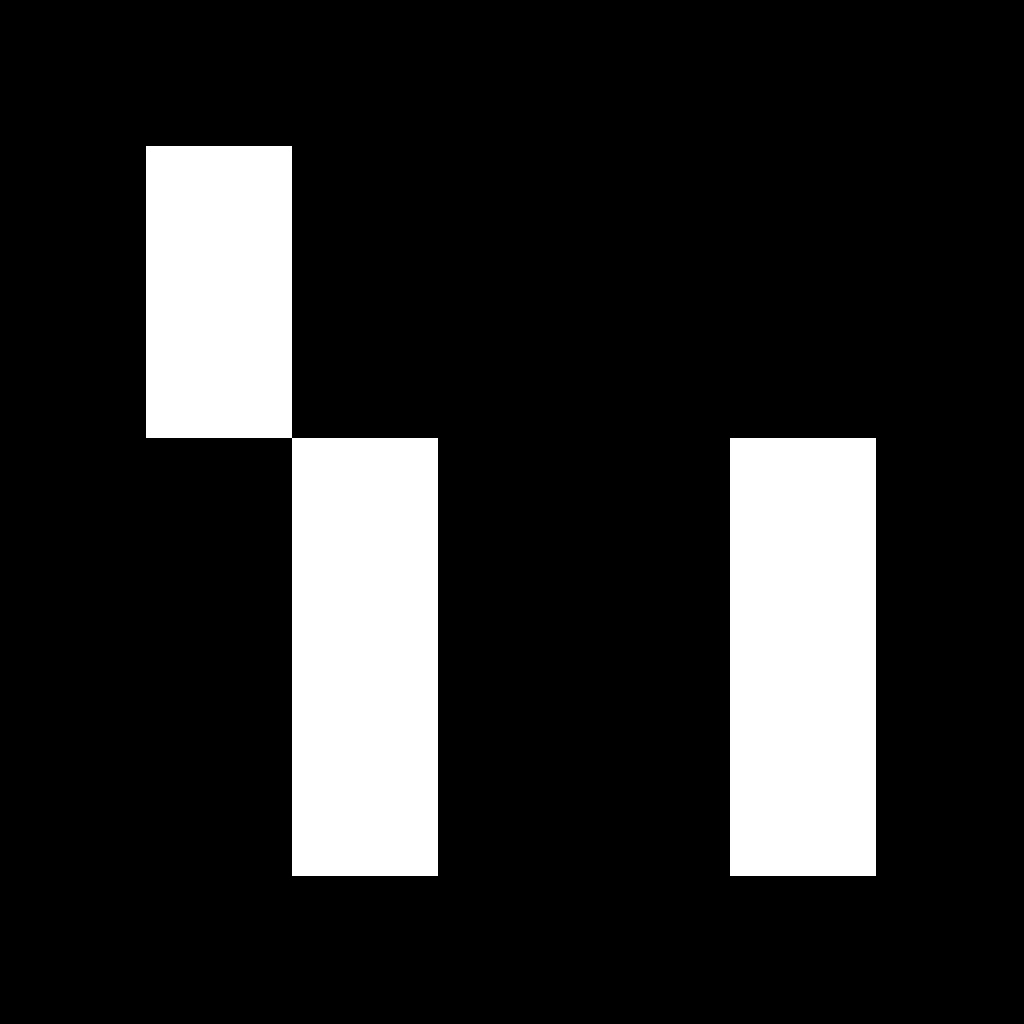
\includegraphics[width=0.8in]{img/42.jpg} &

\includegraphics[width=0.8in]{img/64.jpg}
\end{array}$
\end{center}
\caption{AR codes (10, 23, 25, 42,64)}
\end{figure}

\begin{figure}[h]
\begin{center}$
\begin{array}{ccccc}

\includegraphics[width=0.8in]{img/69.jpg} &

\includegraphics[width=0.8in]{img/116.jpg} &

\includegraphics[width=0.8in]{img/123.jpg} &

\includegraphics[width=0.8in]{img/128.jpg} &

\includegraphics[width=0.8in]{img/256.jpg}
\end{array}$
\end{center}
\caption{AR codes (69, 116, 123, 128, 256)}
\end{figure}

\begin{figure}[h]
\begin{center}$
\begin{array}{ccccc}

\includegraphics[width=0.8in]{img/444.jpg} &

\includegraphics[width=0.8in]{img/456.jpg} &

\includegraphics[width=0.8in]{img/501.jpg} &

\includegraphics[width=0.8in]{img/507.jpg} &

\includegraphics[width=0.8in]{img/512.jpg}
\end{array}$
\end{center}
\caption{AR codes (444, 456, 501, 507, 512)}
\end{figure}

\begin{figure}[h]
\begin{center}$
\begin{array}{ccccc}

\includegraphics[width=0.8in]{img/666.jpg} &

\includegraphics[width=0.8in]{img/789.jpg} &

\includegraphics[width=0.8in]{img/890.jpg} &

\includegraphics[width=0.8in]{img/901.jpg} &

\includegraphics[width=0.8in]{img/999.jpg}
\end{array}$
\end{center}
\caption{AR codes (666, 789, 890, 901,999)}
\end{figure}
\subsubsection{Path-planning}
\subsection{Omgaan met de markers}
Nu kan je makkelijk AR markers vinden in plaatjes, dit maakt de computer vision een stuk makkelijker! Het enige wat je nog nodig hebt is wat de x,y waardes zeggen over de locatie van de marker in de werkelijke 3D ruimte. Dit is natuurlijk nodig om de Nao naar de marker toe te laten lopen. Hiervoor hebben we de functie tools.calcPosition(x\_image,y\_image) in de tools module. Dit is een slimme functie die met behulp van de hoogte informatie van de nao, en de informatie dat de AR code op de grond ligt (!) berekend wat de echte x,y afstand is met als input de x en y waardes uit het plaatje. De functie neemt ook de draaiïng van het hoofd van de Nao mee, dus als de Nao zijn hoofd draait naar een marker dan is de output (x,y) nog steeds precies wat de Nao hoort te lopen om op de marker te komen (jammer genoeg loopt hij niet zo accuraat).

\begin{Exercise}
\begin{itemize}
\item Schrijf nu een functie in een nieuwe dag 3 module waar je een plaatje van de Nao aan mee kan geven, en een lijst met informatie over alle markers teruggeeft. (bijvoorbeeld [(x\_1,y\_1,ID\_1), (x\_1,y\_1,ID\_1)]).
\item Schrijf een functie die het hoofd van de Nao laat draaien naar een marker (input (x\_1,y\_1,ID\_1))
\item Schrijf een functie die een functie op een marker laat lopen.
\item Voeg alle ID markers op nummer toe aan de representatie van het doolhof.
\item Test of al deze functies goed werken!
\end{itemize}
\end{Exercise}
\vspace{10 mm}

\subsection{Volledige autonome navigatie}
Je hebt nu alle tools om de Nao zelfstandig door het doolhof te laten lopen! Met A* kan de Nao een pad plannen, en met de AR markers weet de Nao waar hij is en kan je eenvoudig lopen.

\begin{Exercise}
\begin{itemize}
\item Schrijf nu een main waarbij je zelf een beginpunt en eindpunt op kan geven, de Nao uit zichzelf het pad berekend vanuit het begin naar het einde, en deze dan ook loopt.
\item Probeer je functie uit met verschillende begin en eindpunten, vertel ons of je het werkend hebt gekregen, dat is echt een geweldige prestatie!
\item Als je nog tijd over hebt kan je een Nao zelf uit een doolhof laten lopen vanuit elke positie. De nao word hierbij op een random punt in het doolhof gezet en hij moet zelf bepalen waar hij is, en hoe hij van dat punt naar de opgegeven uitgang moet lopen. Denk er goed over na hoe de Nao kan bepalen waar hij is, en hoe hij gedraaid staat. Wat doe je als de Nao helemaal geen marker ziet?
\end{itemize}
\end{Exercise}
\vspace{10 mm}

\subsection{Tips}

\appendix

\cleardoublepage
\section{Python}
\subsection{Variabelen}
\subsection{Control-statements}
\subsection{Dictionaries en Lijsten}
\subsection{Classes}

\cleardoublepage
\section{Framework}
\subsection{Een Module}
\subsection{De Main-Module}
\subsection{Het Configuratie bestand}

\cleardoublepage
\section{Reference Guide}
\end{document}